\documentclass[12pt]{article}
\usepackage[english]{babel}
\usepackage[utf8x]{inputenc}
\usepackage{amsmath}
\usepackage{graphicx}
\usepackage{graphicx, lipsum,caption}
\usepackage[colorinlistoftodos]{todonotes}

\begin{document}
	
	\begin{titlepage}
		
		\newcommand{\HRule}{\rule{\linewidth}{0.5mm}} % Defines a new command for the horizontal lines, change thickness here
		
		\center % Center everything on the page
		
		%----------------------------------------------------------------------------------------
		%	HEADING SECTIONS
		%----------------------------------------------------------------------------------------
		
		\textsc{\LARGE Central Washington University}\\[1.5cm] % Name of your university/college
		\textsc{\Large Advanced Algorithms}\\[0.5cm] % Major heading such as course name
		\textsc{\large Winter 2019}\\[0.5cm] % Minor heading such as course title
		
		%----------------------------------------------------------------------------------------
		%	TITLE SECTION
		%----------------------------------------------------------------------------------------
		
		\HRule \\[0.4cm]
		{ \huge \bfseries Project 4 Report}\\[0.4cm] % Title of your document
		\HRule \\[1.5cm]
		
		%----------------------------------------------------------------------------------------
		%	AUTHOR SECTION
		%----------------------------------------------------------------------------------------
		
		\begin{minipage}{0.4\textwidth}
			\begin{flushleft} \large
				\emph{Author:}\\
				Hermann \textsc{Yepdjio} % Your name
			\end{flushleft}
		\end{minipage}
		~
		\begin{minipage}{0.4\textwidth}
			\begin{flushright} \large
				\emph{Professor:} \\
				Dr. Razvan \textsc{Andonie} % Supervisor's Name
			\end{flushright}
		\end{minipage}\\[1cm]
		
		% If you don't want a supervisor, uncomment the two lines below and remove the section above
		%\Large \emph{Author:}\\
		%John \textsc{Smith}\\[3cm] % Your name
		
		%----------------------------------------------------------------------------------------
		%	DATE SECTION
		%----------------------------------------------------------------------------------------
		
		{\large \today}\\ % Date, change the \today to a set date if you want to be precise
		
		%----------------------------------------------------------------------------------------
		%	LOGO SECTION
		%----------------------------------------------------------------------------------------
		
		
\includegraphics[width=12cm]{CWU-Logo.png}\\[.5cm] % Include a department/university logo - this will require the graphicx package
		
		%----------------------------------------------------------------------------------------
		
		\vfill % Fill the rest of the page with whitespace
		
	\end{titlepage}
	\newpage
	\tableofcontents
	\newpage
	
	
	
	\section{Introduction}
		The purpose of this project was to experiment using the RSA public-key cryptosystem to encrypt and decrypt messages and Pollard-Rho's algorithm to break encryption codes. We experimented using different large prime numbers for p and q. The details and results of the experimentation are discussed below. 
	\section {experimentation process}
	    \subsection{Self Experimentation}
			we experimented using primes of k bits ( k = 30, 35, 40,...,55). The program uses Miller-Rabin's algorithm to check if the numbers are primes. we stopped at 55 because the pollard-rho implementation would take forever to factor the modulus if we were going beyond that. 
			The experimentation starts with the user inputting a message to be encrypted. Then, for each value of k, we do the following:
			\begin{itemize}
				\item generate both a private-key and a public-key following the RSA public-key cryptosystem algorithm from the book 
				\item using the public-key, we encrypt the message and record how long it takes,
				\item using the the private-key, we decrypt the message and record how long it takes ,
				\item using the public-key, we try to decrypt the message and record how long it takes,
			\end{itemize}
		\subsection{Experimenting with a Classmate}
			For this part of the experiment, I teamed with Brian. I was able to break his code in about 7 seconds and he was also able to break mine.
	\section{Results}
		The results of the experimentation are contained in the table below
		
		
		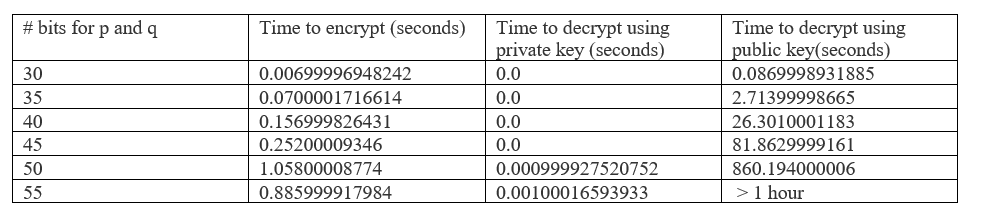
\includegraphics[width=15cm]{result.PNG}\\[.5cm]	
		
		As we can see from the table above, 
		\begin{itemize}
			\item the time spent for encrypting a message increases very slowly as the number of bits for p and q increases
			\item the time spent for decrypting a cipher-text using the private key is really small and increases extremely slowly as the number id bits for p and q increases
			\item the time spent for decrypting a cipher-text using the public key is big and increases really fast as the number of bits for p and q increases
		\end{itemize}
		
	\section{Conclusion}
		From the experimentation above, we observed that increasing the values of p and q makes the encryption code harder to break. Since both encrypting and decrypting using the private key are fast, it makes therefore more sense to use very large values for p and q to produce the keys as it only really affect the people who might try to break the encryption code.
		
	
\end{document}
